%% CIShell Algorithm Developer's Guide
%%
%

\documentclass[pdftex,11pt,a4paper]{article}
\usepackage[top=0.4in, left=0.5in, right=0.5in, bottom=0.6in]{geometry}
\usepackage[pdftex]{graphicx}
\DeclareGraphicsExtensions{.pdf,.png,.jpg,.mps,.eps}
\usepackage[pdftex]{hyperref}
\usepackage{color}

\hypersetup{
    pdftitle={CIShell Algorithm Developer's Guide},    % title
    pdfsubject={CIShell Algorithm Developer's Guide},
    pdfauthor={},      
    pdfnewwindow=true,      % links in new window
}

\usepackage[refpages]{gloss}
\renewcommand{\glosslinkborder}{0 0 0}
\renewcommand{\glosslinkcolor}{blue}

\makegloss

\usepackage{../mystyle}

\title{CIShell Algorithm Developer's Guide \\
\textbf{DRAFT}}
% \author{} % Will fill in later 
% \date{} % ditto

\begin{document}

\maketitle{}
\tableofcontents{}


% Overview, introduction, etc.
\section{CIShell Core Overview}
\subsection{Introduction}
\subsection{Concepts}
\subsection{GUI}

\section{Plugin Tutorials}
% Setup
\subsection{Setting Up the Environment}

% General Algs
\subsection{General Algorithm Development}
\subsubsection{Concepts}

\gloss[Long]{osgi} and stuff.

\begin{figure}[htb!]
\centering
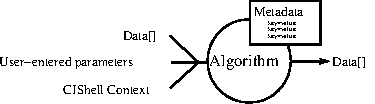
\includegraphics[width=90mm]{../img/algorithmDefn.pdf}
\caption{Algorithm Definition}
\label{fig:algorithmDefn}
\end{figure}


\subsubsection{Java-based}
\subsubsection{Static-Executable}
\subsubsection{Jython-based}

% Specific Algs
\subsection{Specific Algorithm types}
\subsubsection{Analysis}
\subsubsection{Modeling}

\subsubsection{Visualizations}
\subsubsection{Sample Data}
\subsubsection{Data Loading And Conversion}

\paragraph{Introduction}
\paragraph{Supporting New File Types}
\paragraph{Converters}


% Other Tutorials
\subsection{Java Libraries}
\subsection{Available Services}

\subsection{Creating GUIs}

% Software Update Tool
\section{Software Update Tool}
\subsection{Using the Software Update Tool}

\subsection{Creating an Update Site}
\subsubsection{Features}
\subsubsection{Update Site}

\section{Appendix}
\subsection{Accessing Exemplary Algorithms}

\subsection{Accessing CIShell-Related Update Sites}


\printgloss{../glossary}

% Bibliography:
\clearpage
\bibliographystyle{plain}
\bibliography{../bibliography}

\end{document}
